\documentclass{article}
\usepackage[dvipsnames]{xcolor}
\usepackage[paperwidth=12cm, paperheight=12cm, margin = 0cm, top=0.5cm]{geometry}
\usepackage{amsmath}


\usepackage{pgf}
\usepackage{tikz}


\usetikzlibrary{arrows,automata, positioning}

\tikzstyle{source}  = [draw,circle,fill=black,thick,inner sep=0mm,minimum size=2mm]

\renewcommand{\vec}[1]{\boldsymbol{#1}}

\begin{document}
\begin{center}
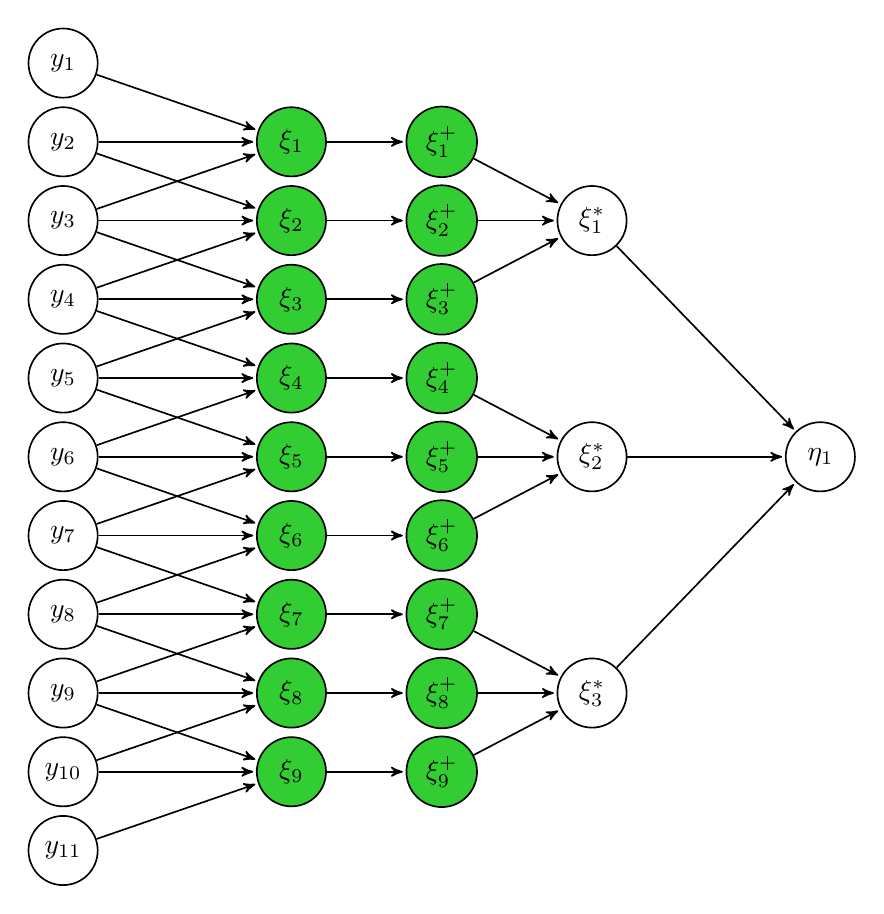
\begin{tikzpicture}[-,>=stealth',shorten >=1pt,auto,node distance=1cm,semithick]
                    
\node[state] (Y1)               {$y_{1}$}; 
\node[state] (Y2) [below of=Y1] {$y_{2}$};                   
\node[state] (Y3) [below of=Y2] {$y_{3}$};                   
\node[state] (Y4) [below of=Y3] {$y_{4}$};                   
\node[state] (Y5) [below of=Y4] {$y_{5}$};                   
\node[state] (Y6) [below of=Y5] {$y_{6}$};                   
\node[state] (Y7) [below of=Y6] {$y_{7}$};                   
\node[state] (Y8) [below of=Y7] {$y_{8}$};                   
\node[state] (Y9) [below of=Y8] {$y_{9}$}; 
\node[state] (Y10) [below of=Y9] {$y_{10}$};                   
\node[state] (Y11) [below of=Y10] {$y_{11}$}; 

\node[state, fill=LimeGreen] (X1) [right=2cm of Y2] {$\xi_{1}$}; 
\node[state, fill=LimeGreen] (X2) [right=2cm of Y3] {$\xi_{2}$}; 
\node[state, fill=LimeGreen] (X3) [right=2cm of Y4] {$\xi_{3}$}; 
\node[state, fill=LimeGreen] (X4) [right=2cm of Y5] {$\xi_{4}$}; 
\node[state, fill=LimeGreen] (X5) [right=2cm of Y6] {$\xi_{5}$}; 
\node[state, fill=LimeGreen] (X6) [right=2cm of Y7] {$\xi_{6}$}; 
\node[state, fill=LimeGreen] (X7) [right=2cm of Y8] {$\xi_{7}$}; 
\node[state, fill=LimeGreen] (X8) [right=2cm of Y9] {$\xi_{8}$}; 
\node[state, fill=LimeGreen] (X9) [right=2cm of Y10] {$\xi_{9}$}; 

\node[state, fill=LimeGreen] (XP1) [right=1cm of X1] {$\xi_{1}^+$}; 
\node[state, fill=LimeGreen] (XP2) [right=1cm of X2] {$\xi_{2}^+$}; 
\node[state, fill=LimeGreen] (XP3) [right=1cm of X3] {$\xi_{3}^+$}; 
\node[state, fill=LimeGreen] (XP4) [right=1cm of X4] {$\xi_{4}^+$}; 
\node[state, fill=LimeGreen] (XP5) [right=1cm of X5] {$\xi_{5}^+$}; 
\node[state, fill=LimeGreen] (XP6) [right=1cm of X6] {$\xi_{6}^+$}; 
\node[state, fill=LimeGreen] (XP7) [right=1cm of X7] {$\xi_{7}^+$}; 
\node[state, fill=LimeGreen] (XP8) [right=1cm of X8] {$\xi_{8}^+$}; 
\node[state, fill=LimeGreen] (XP9) [right=1cm of X9] {$\xi_{9}^+$}; 

\node[state] (XM1) [right=1cm of XP2] {$\xi_{1}^*$};                   
\node[state] (XM2) [right=1cm of XP5] {$\xi_{2}^*$};                   
\node[state] (XM3) [right=1cm of XP8] {$\xi_{3}^*$};                   

\node[state] (Z1) [right=2cm of XM2] {$\eta_{1}$};                     


\path (Y1) edge[->] (X1)
      (Y2) edge[->] (X1)
      (Y3) edge[->] (X1)
      (Y2) edge[->] (X2)
      (Y3) edge[->] (X2)
      (Y4) edge[->] (X2)
      (Y3) edge[->] (X3)
      (Y4) edge[->] (X3)
      (Y5) edge[->] (X3)
      (Y4) edge[->] (X4)
      (Y5) edge[->] (X4)
      (Y6) edge[->] (X4)
      (Y5) edge[->] (X5)
      (Y6) edge[->] (X5)
      (Y7) edge[->] (X5)
      (Y6) edge[->] (X6)
      (Y7) edge[->] (X6)
      (Y8) edge[->] (X6)
      (Y7) edge[->] (X7)
      (Y8) edge[->] (X7)
      (Y9) edge[->] (X7)
      (Y8) edge[->] (X8)
      (Y9) edge[->] (X8)
      (Y10) edge[->] (X8)
      (Y9) edge[->] (X9)
      (Y10) edge[->] (X9)
      (Y11) edge[->] (X9);
      
\path (X1) edge[->] (XP1)
      (X2) edge[->] (XP2)
      (X3) edge[->] (XP3)
      (X4) edge[->] (XP4)
      (X5) edge[->] (XP5)
      (X6) edge[->] (XP6)
      (X7) edge[->] (XP7)
      (X8) edge[->] (XP8)
      (X9) edge[->] (XP9);

\path (XP1) edge[->] (XM1)
      (XP2) edge[->] (XM1)
      (XP3) edge[->] (XM1)
      (XP4) edge[->] (XM2)
      (XP5) edge[->] (XM2)
      (XP6) edge[->] (XM2)
      (XP7) edge[->] (XM3)
      (XP8) edge[->] (XM3)
      (XP9) edge[->] (XM3);
      
\path (XM1) edge[->] (Z1)
      (XM2) edge[->] (Z1)
      (XM3) edge[->] (Z1);
      
\end{tikzpicture}
\end{center}

\end{document}
